\cotefile{148}
\scanpage{14}

\noindent
\begin{minipage}[t]{.43\linewidth}
\centering\small
U N I V E R S I T E\\
DES SCIENCES ET TECHNIQUES\\
DU LANGUEDOC\\
\texttt{-{}-{}-{}-{}-{}-{}-{}-{}-{}-{}-{}-}

Service de la Scolarité\\
MA/GJ\\
Diffusion : Liste A\\
N°: 4680
\end{minipage}\hfill
\begin{minipage}[t]{.53\linewidth}
\small\vspace{2\baselineskip}
Montpellier, le 20 octobre 1983
\end{minipage}

\begin{center}
\uline{AVIS DE SOUTENANCE D'UNE THESE DE DOCTORAT DE 3ème CYCLE}

\uline{EVOLUTION ET BIOSYSTEMATIQUE}
\end{center}

\uline{Nom et prénom de la candidate} : CHAKROUN Sa\unsure{\={\i}|ï}da

\uline{Titre de la thèse} : LES VARIATIONS SAISONNIERES DES FORMATIONS SECONDAIRES (BOIS, LIBER, CAMBIUM) DU TRONC DE TROIS ESPECES MEDITERRANEENNES, LE CHENE VERT, L'OLIVIER, ET LE MICOCOULIER : UNE ETUDE HISTOPHYSIOLOGIQUE.

\uline{Date, heure et lieu de soutenance prévus} : 28 Octobre 1983 à 9h30\\
Salle de Cours n°9 - U.S.T.L.

\uline{Nom des Directeurs de thèse} : MM. Charles HEBANT et BONNET

\uline{Désignation du laboratoire où la thèse est préparée} : Laboratoire de Biologie Végétale

\uline{Résumé de la thèse} :

Cette étude concerne l'anatomie, l'histologie et l'histo-\\
chimie des tissus conducteurs secondaires d'\textit{Olea europaea}, de \textit{Quercus ilex}, et de \textit{Celtis australis}.

Le bois et le liber du Chêne et de l'Olivier ont fait l'objet d'une étude structurale approfondie.

Le fonctionnement de la zone cambiale (ainsi que la mise en place de ses dérivés, bois et liber) et l'évolution des réserves amylacées du tronc de ces trois espèces subissent des variations importantes avec le rythme saisonnier, et dans le cas de l'Olivier, avec les alternances de production.

Chez le Chêne et le Micocoulier, la totalité du bois et du liber est différenciée au printemps et en été. Chez l'Olivier, la réactivation cambiale au printemps est plus ou moins précoce selon la charge en fruits ; de plus, seuls les arbres en faible production montrent une reprise d'activité cambiale en automne, cette dernière engendre uniquement du bois.

Chez les trois espèces, la mise en place du liber est initiée plus tardivement que dans le cas du bois. Chez les deux espèces à feuilles persistantes, la zone du liber conducteur ne disparaît jamais, par contre, chez le Micocoulier, à la fin de l'automne et pendant l'hiver, tous les tubes criblés deviennent non conducteurs en accumulant de la callose.

Parallèlement à la réactivation cambiale, on note une hydro-\\
lyse de l'amidon. L'amylogénèse est plus ou moins précoce selon l'espèce observée, et dans le cas de l'Olivier, selon la charge en fruits. Une compétition entre la croissance végé-\\
tative et le développement reproductif de l'Olivier est observée.

Tout au long de l'année, les cellules compagnes et les rayons vasculaires du Chêne et de l'Olivier possèdent une forte activité phosphohydrolasique et respiratoire.

\uline{Durée approximative des recherches ayant abouti à la thèse} : 3 ans

\uline{Composition du jury proposée} :

\begin{tabular}{ll}
MM. & D'AUZAC J.\\
& BONNET A.L.\\
& KAUMAN W.\\
& NABLI M.A\\
& THALER L.\\
& VILLEMUR P.
\end{tabular}

% Closing typescript with the autograph contours in their overlapping positions.
% The signature's alphabetic reading remains undecided.
\figure{%
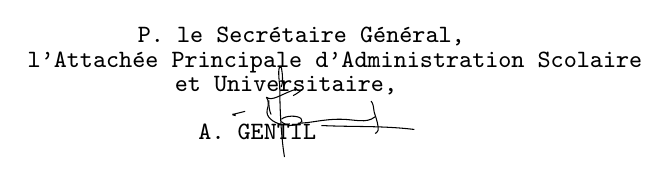
\begin{tikzpicture}[x=.01cm,y=-.01cm,line width=.38pt,
  every node/.style={font=\ttfamily\fontsize{9}{11}\selectfont,inner sep=0pt}]
  \node[anchor=base west] at (154,4) {P. le Secrétaire Général,};
  \node[anchor=base west] at (14,35) {l'Attachée Principale d'Administration Scolaire};
  \node[anchor=base west] at (201,66) {et Universitaire,};
  \node[anchor=base west] at (231,127) {A. GENTIL};
  % SIGNATURE_INK_BEGIN
  \draw (275,95) -- (291,91);
  \draw[line width=.6pt] (275,95) -- (279,96);
  \draw (337,35) .. controls (333,31) and (333,44) .. (335,58)
    .. controls (335,90) and (337,125) .. (341,149);
  \draw (337,35) .. controls (339,46) and (339,55) .. (337,60);
  \draw (318,73) .. controls (321,77) and (321,83) .. (319,89)
    .. controls (317,98) and (326,105) .. (338,108);
  \draw (321,77) .. controls (321,85) and (322,91) .. (324,95);
  \draw (318,73) .. controls (325,79) and (337,69) .. (355,63);
  \draw (352,71) .. controls (358,68) and (361,65) .. (364,63);
  \draw (337,101) .. controls (343,96) and (357,96) .. (362,100)
    .. controls (367,105) and (357,109) .. (347,109);
  \draw (337,104) .. controls (341,108) and (345,108) .. (348,107);
  \draw (358,106) .. controls (375,106) and (388,101) .. (412,101)
    .. controls (430,101) and (445,107) .. (456,98);
  \draw (451,78) .. controls (454,81) and (454,86) .. (455,92)
    .. controls (458,101) and (461,111) .. (460,115)
    .. controls (459,118) and (457,119) .. (456,119);
  \draw (388,109) .. controls (430,111) and (464,109) .. (506,114);
  % Editorial marker for the undecided alphabetic reading.
  \node[anchor=base west] at (520,114) {\unsure{\phantom{A}}};
  % SIGNATURE_INK_END
\end{tikzpicture}%
}

\margin{13}
